\documentclass[aspectratio=169, 8pt, xcolor={svgnames}, hyperref={linkcolor=black}]{beamer}
\usepackage[labelfont={color=amethyst,bf}]{caption}
\setbeamercolor{background canvas}{bg=white}
\usetheme[progressbar=frametitle]{metropolis}
\usepackage{appendixnumberbeamer}
\usepackage{url}
\usepackage{booktabs}
\usepackage{braket}
\usepackage[scale=2]{ccicons}
\usepackage{amsfonts} 
\usepackage{amssymb}
\usepackage[english]{babel}
\colorlet{col1}{teal}
\colorlet{col2}{yellow}
\colorlet{col3}{green}
\usepackage{fontawesome}
\usepackage{subcaption}
\usepackage{multicol}
\usepackage{bm}
\usepackage{algorithm}
\usepackage{overpic}
\usepackage{algpseudocode}
\usepackage{enumitem}

\usepackage[]{pseudo}


\usepackage{tikz}
\usetikzlibrary{positioning,arrows,calc,math,angles,quotes}
\usepackage{blochsphere}


\usetikzlibrary{arrows,automata}
\usetikzlibrary{positioning}
\usetikzlibrary{arrows.meta,
                bending,
                intersections,
                quotes,
                shapes.geometric}

\tikzset{
    state/.style={
           rectangle,
           rounded corners,
           draw=black, very thick,
           minimum height=1em,
           inner sep=2pt,
           text centered,
           },
}


\definecolor{myv}{rgb}{0.36, 0.22, 0.33}
\definecolor{gio}{rgb}{0.45, 0.31, 0.59}
\definecolor{light}{rgb}{0.8, 0.8, 1}
\definecolor{warmblack}{rgb}{0.0, 0.26, 0.26}
\definecolor{brown(web)}{rgb}{0.65, 0.16, 0.16}
\definecolor{cadmiumgreen}{rgb}{0.0, 0.42, 0.24}
\definecolor{darkmidnightblue}{rgb}{0.0, 0.2, 0.4}
\definecolor{brightube}{rgb}{0.82, 0.62, 0.91}

\definecolor{codegreen}{rgb}{0,0.6,0}
\definecolor{codegray}{rgb}{0.5,0.5,0.5}
\definecolor{codepurple}{rgb}{0.58,0,0.82}
\definecolor{backcolour}{rgb}{0.95,0.95,0.92}
\definecolor{amethyst}{rgb}{0.6, 0.33, 0.73}

\definecolor{light-gray}{gray}{0.95}
\newcommand{\code}[1]{\colorbox{light-gray}{\texttt{#1}}}


\usepackage{listings}
\lstdefinestyle{mystyle}{
    backgroundcolor=\color{backcolour},   
    commentstyle=\color{codegreen},
    keywordstyle=\color{codepurple},
    numberstyle=\tiny\color{codepurple},
    stringstyle=\color{magenta},
    basicstyle=\footnotesize,
    breakatwhitespace=false,         
    breaklines=true,                 
    captionpos=b,                    
    keepspaces=true,                 
    numbers=left,                    
    numbersep=5pt,                  
    showspaces=false,                
    showstringspaces=false,
    showtabs=false,                  
    tabsize=2
}

\lstset{style=mystyle}
\usepackage[most]{tcolorbox}
\usepackage{xcolor}


%\usepackage[citecolor = green, linkcolor = blue, bookmarks=true, urlcolor=blue,
%colorlinks=true, pagebackref=true]{hyperref}


%\usepackage{xspace}

\title{Ancillary qubits}
\subtitle{Quantum Computing Minicourse ICTP-SAIFR}
\date{8 April 2024}
\author{Stefano Carrazza$^\ddag$ and Matteo Robbiati$^\dagger$}
\institute{$^\ddag$ Associate Professor \& Researcher, University of Milan and INFN Milan, Italy.\\
$^\dagger$ PhD candidate, University of Milan, Italy and CERN, Switzerland.}
\titlegraphic{
\begin{tikzpicture}[overlay, remember picture]

\node[at=(current page.south), anchor=south, shift={(-3cm, 0)}] {%
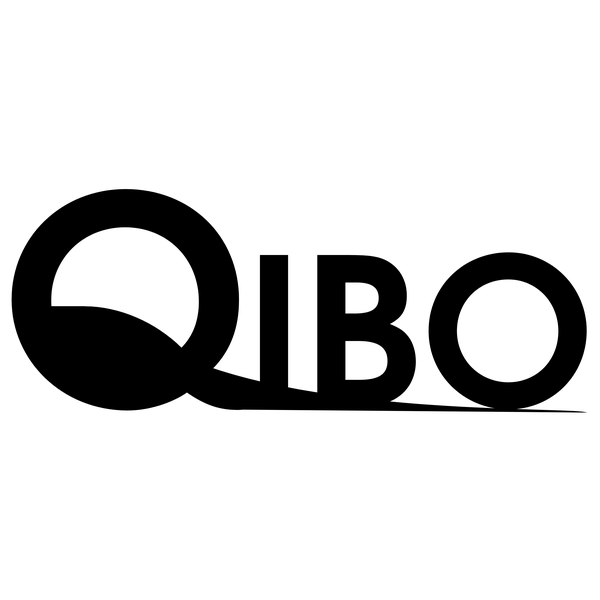
\includegraphics[width=.12\textwidth]{figures/qibo.png}

\includegraphics[width=.12\textwidth]{figures/unimi.png}

\includegraphics[width=.12\textwidth]{figures/cern.png}

\includegraphics[width=.12\textwidth]{figures/ictp.png}
};
\end{tikzpicture}
}


\begin{document}

\begin{frame}
\maketitle
\begin{picture}(0,0)
    \put(270,20){
        
\includegraphics[width=0.3\textwidth]{figures/qibo_boomerang.png}
    }
\end{picture}
\end{frame}

\begin{frame}{Ancillary qubits}
\textbf{Ancilla} qubits are extra qubits, which help a qubit system in some computations.   
For example:
   \begin{figure}
     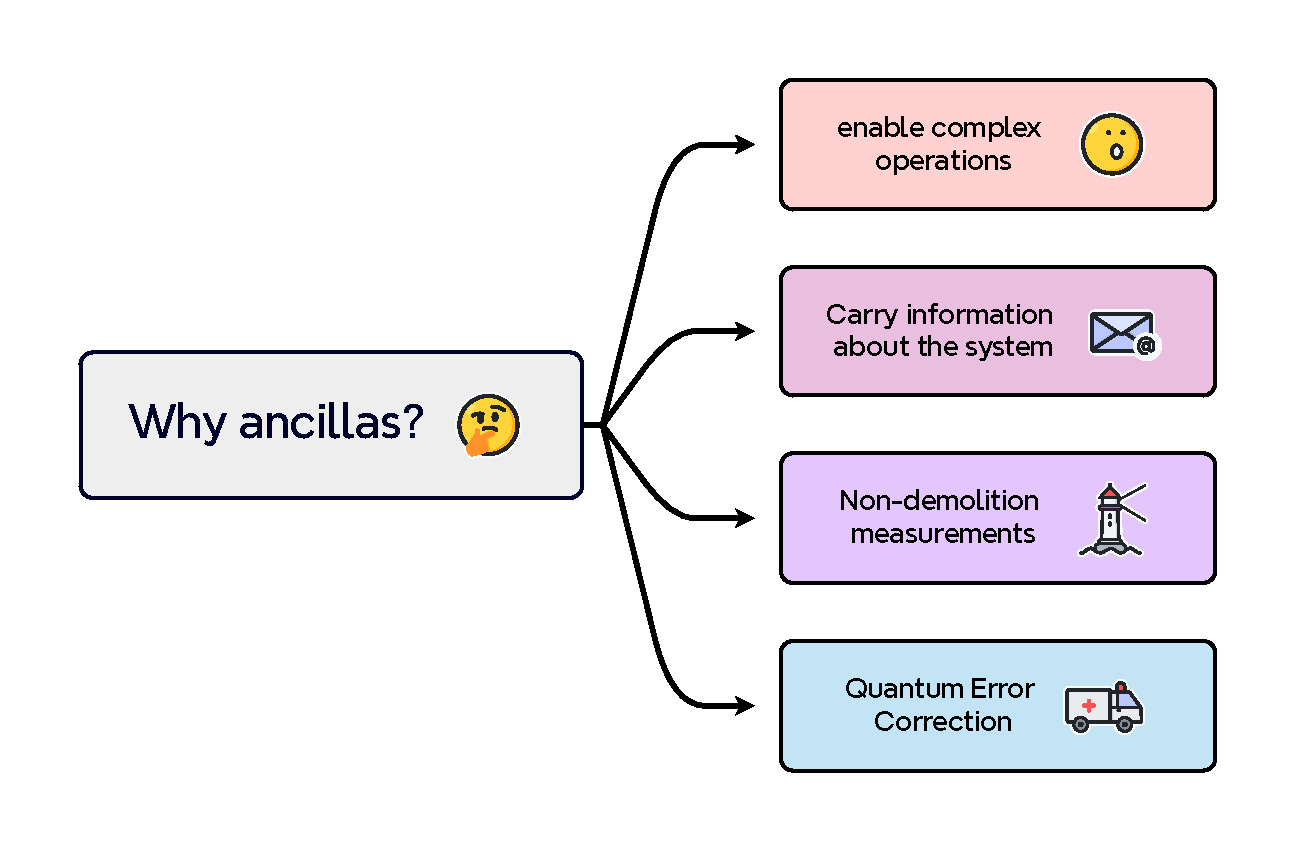
\includegraphics[width=0.75\linewidth]{figures/ancillas.pdf}
   \end{figure}
\end{frame}

\begin{frame}{The phase kickback}
One clever trick we can implement using ancillas is the \textbf{phase kickback}.
\pause

\begin{itemize}[noitemsep]
\item{1.} Take into account two qubits: a system qubit $x$ and an ancilla $y$.  \pause
\item{2.} Suppose we prepare $x$ into a superposed state and $y$ into the excited state:
$$ \ket{x}=H\ket{0} = \frac{\ket{0}+\ket{1}}{\sqrt{2}}, \qquad \ket{y}=\ket{1}. $$ \pause
\item{3.} Let's consider now a controlled $Z$ operation. \pause
\item{4.} What happen if we now apply the $CZ$ using $x$ as control and $y$
as target? \pause
\item{5.} we could expect something happen on the target qubit! Not really: \pause
$$ CZ \biggl( \frac{\ket{0}+\ket{1}}{\sqrt{2}} \otimes \ket{1} \biggr)  = 
CZ \biggl( \frac{\ket{01}+\ket{11}}{\sqrt{2}} \biggr) = \pause
\frac{\ket{01}+Z\ket{11}}{\sqrt{2}} = \pause
\frac{\ket{01}-\ket{11}}{\sqrt{2}} = \pause
\frac{\ket{0}-\ket{1}}{\sqrt{2}} \otimes \ket{1}.
$$ \pause
\item{6.} adding an extra $H$ to the control qubit, we will detect the state manipulation!
\end{itemize}

\pause
\begin{tcolorbox}[colback=red!15, title=Important]
This happens if the ancilla is prepared into a state which is eigenvector of the 
controlled operation.
\end{tcolorbox}

\end{frame}

\begin{frame}{Is the phase kickback useful?}
Some of the most powerful and famous quantum computing algorithms make use of the phase kickback
\begin{multicols}{4}
\begin{figure}
   {
\includegraphics[width=0.23\textwidth, height=0.4\textheight]{figures/dj.png}\caption{Deutsch-Josza}}
   {
\includegraphics[width=0.23\textwidth, height=0.4\textheight]{figures/grover.png}\caption{Grover}}
   {
\includegraphics[width=0.23\textwidth, height=0.4\textheight]{figures/shor.png}\caption{Shor}}
   {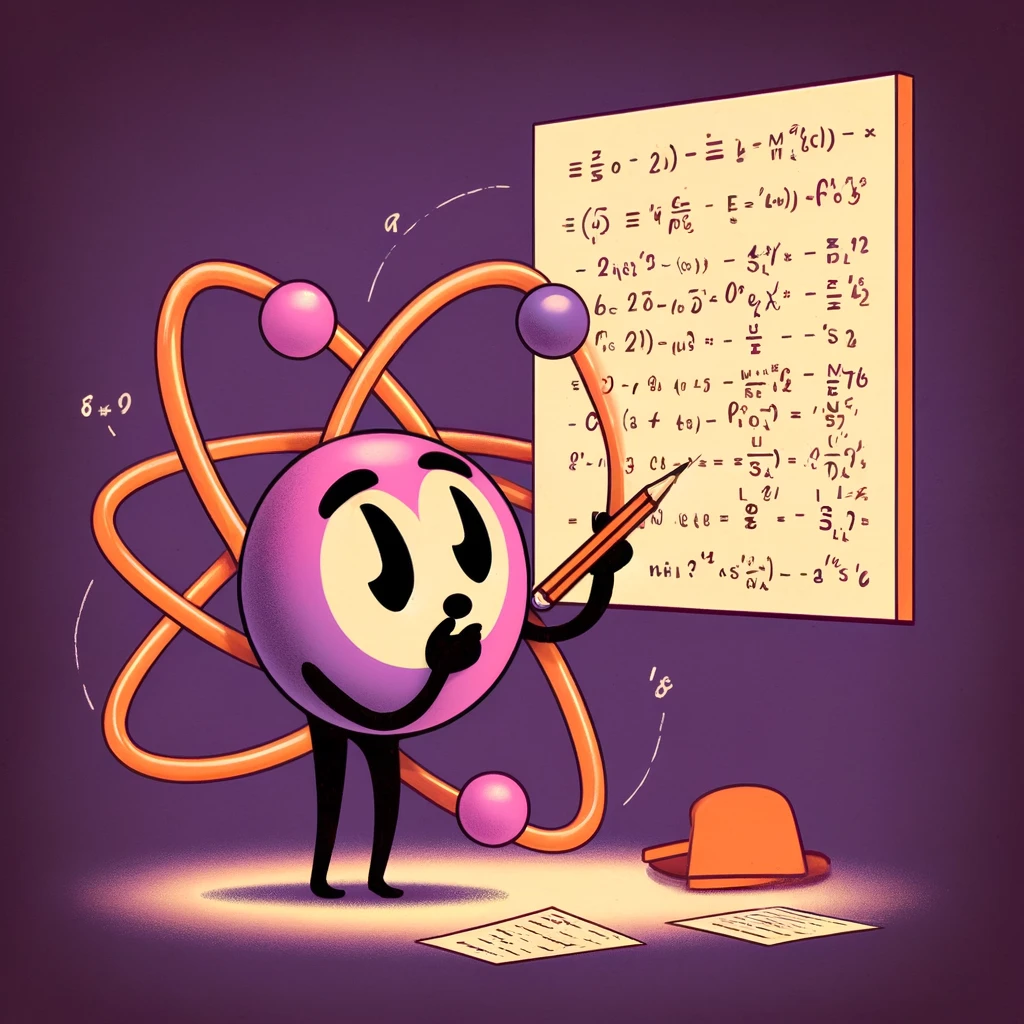
\includegraphics[width=0.23\textwidth, height=0.4\textheight]{figures/hhl.png}\caption{HHL}}
\end{figure}
\end{multicols}
All of them are proved to outperform any classical algorithm, leading to a theoretical \textbf{quantum 
advantage}!
\end{frame}

\begin{frame}{Oracles}
It can be useful to define the phase kickback using the concept of quantum \textbf{oracle}.

\begin{itemize}[noitemsep]
\item[1.] Considering a system of qubits of state $\ket{x}$ and a set of extra qubits of state $\ket{y}$; \pause
\item[2.] in reversible computation $x$ is called \textbf{input register} and $y$ \textbf{output register}. In this 
course $x$ will always be composed of our system of qubits and $y$ will be ancillary qubits; \pause
\item[3.] considering a function $f(x)$, acting on $y$, we define 
oracle $U_f$, a \textbf{black box} operator whose action on $\ket{y}$ is:
\begin{figure}
   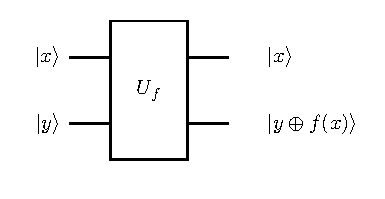
\includegraphics[width=0.4\textwidth]{figures/oracle.pdf}
\end{figure}
\pause
\end{itemize}
In the explicit case of the phase kickback, we can use $U_f$ to write the action: $U_f \ket{x}\ket{-} = (-1)^{x}\ket{x}\ket{-}.$\pause

Extending it to a multi-dimensional case, we can write: $U_f \ket{x}\ket{-} = (-1)^{f(x)}\ket{x}\ket{-},$ whith $f(x) \in \{0,1\}$.
\end{frame}

\begin{frame}
\centering
\Huge Let's code!
\begin{figure}
   
\includegraphics[width=0.7\textwidth]{figures/hands_on.png}
\end{figure}
\end{frame}


\end{document}
